\section{Μεθοδολογία υλοποίησης} \label{subsection:4-1-implementation-methodology}

Για την επίτευξη των στόχων που ορίστηκαν και την οργάνωση της εργασίας που απαιτείται σε διαχειρίσιμα μέρη, σχεδιάστηκε η χρήση διάφορων εργαλείων και μεθόδων ανάπτυξης λογισμικού, όπως το σύστημα ελέγχου εκδόσεων (version control system) Git, η μέθοδος οργάνωσης Scrum και οι διαδικασίες ανάπτυξης DevOps. Τα εργαλεία αυτά είναι δοκιμασμένα και έχουν εδραιωθεί στη σύγχρονη ανάπτυξη λογισμικού.

Μέσα από την χρήση των παραπάνω εργαλείων επιτυγχάνεται η ομαλή συνεργασία στην ανάπτυξη του λογισμικού. Κάθε μέλος της ομάδας δύναται να εργαστεί ανεξάρτητα και χωρίς την ανάγκη διαρκούς επικοινωνίας με τα υπόλοιπα μέλη. Οι στόχοι είναι ορισμένοι, σαφείς και χωρισμένοι σε διαχειρίσιμα μέρη τα οποία δεν καταβάλουν τα μέλη. Ταυτόχρονα, έχοντας ως έδρα καθιερωμένα πρότυπα ανάπτυξης, παρέχεται φορμαλισμός και έτοιμες μέθοδοι επίλυσης προβλημάτων, γεγονός που λειτουργεί καταλυτικά και βοηθά στην αποφυγή τελμάτων κατά τη συγγραφή του κώδικα.

Το Git είναι δωρεάν λογισμικό ανοιχτού κώδικα το οποίο επιτρέπει και επικουρεί την απρόσκοπτη ανάπτυξη λογισμικού από πολλαπλά μέλη μίας ομάδας, ταυτόχρονα και διανεμημένα. Αυτό επιτυγχάνεται παρέχοντας ένα πλαίσιο από εργαλεία τα οποία βοηθούν την διαχείριση και ενσωμάτωση των διαφορετικών εκδόσεων του κώδικα τις οποίες αναπτύσσει κάθε μέλος της ομάδας ξεχωριστά. Υπάρχουν διάφορα μοντέλα χρήσης του Git και πιο συγκεκριμένα της δυνατότητας που δίνει για δημιουργία, ανάπτυξη και ένωση (merge) κλαδιών (branches).

Για τους σκοπούς της παρούσας διπλωματικής χρησιμοποιήθηκε το μοντέλο GitHub flow\cite{4.1-github-flow}. Το μοντέλο αυτό ορίζει ότι κάθε προγραμματιστής ανοίγει ένα νέο branch για τη ανάπτυξη ενός χαρακτηριστικού της εφαρμογής ή τη διόρθωση ενός μέρους του κώδικα. Έπειτα, όταν η δουλειά έχει ολοκληρωθεί, δημιουργείται ένα αίτημα ένωσης (pull request) με το βασικό κλαδί ανάπτυξης (develop) της εφαρμογής. Η δουλειά υπόκειται σε αξιολόγηση από την υπόλοιπη ομάδα (review) και όταν κριθεί ότι ικανοποιεί τις ανάγκες του έργου, το branch γίνεται merge με το develop. Όταν το develop φτάσει σε ικανό σημείο σταθερότητας και αλλαγών, γίνεται merge με το branch παραγωγής (master). Από το master δημιουργούνται οι τελικές εκδόσεις της εφαρμογής οι οποίες διανέμονται για χρήση στην παραγωγή (production versions), ενώ από το develop δημιουργούνται οι δοκιμαστικές εκδόσεις αιχμής της εφαρμογής οι οποίες χρησιμοποιούνται κατά τον έλεγχο (staging versions).

Το Scrum είναι μία μέθοδος οργάνωσης στην οποία ο επιμελητής του Scrum (Scrum master) διαχωρίζει τα ανεξάρτητα μέρη εργασίας (tasks) που πρέπει να υλοποιηθούν για την ολοκλήρωση των στόχων ενός project. Τα μέρη αυτά περιγράφονται αναλυτικά μαζί με τις απαιτήσεις τους και κατατίθενται σε μία λίστα εργασιών (backlog). Έπειτα, μέσα από συσκέψεις (meetings), επιλέγεται ένας αριθμός από tasks τα οποία ορίζουν το επόμενο προγραμματιστικό κύκλο (sprint). Κάθε task ανατίθεται σε κάποιο μέλος για υλοποίηση. Για το Sprint ορίζεται μία χρονική διάρκεια, στόχος της οποίας είναι η περάτωση όλων των tasks πριν τη λήξη της. Στο τέλος της προθεσμίας που ορίστηκε για το Sprint τα μέλη της ομάδας αποτιμούν τα αποτελέσματα και ορίζουν το επόμενο Sprint. Η διαδικασία επαναλαμβάνεται έως ότου το έργο ολοκληρωθεί.

Λόγω του πολύ μικρού μεγέθους της ομάδας, το Scrum ακολουθήθηκε ελαστικά. Συγκεκριμένα, δεν ορίστηκε ένας συγκεκριμένος επιμελητής του board αλλά κάθε μέλος της ομάδας φρόντιζε για τον ορισμό και την περιγραφή ενός μέρους των tasks. Τα sprints δεν ήταν συνεχόμενα και δεν είχαν πάντα τον ίδιο χρόνο εκτέλεσης αλλά προσαρμόζονταν ανάλογα με τις εκάστοτε ανάγκες και τον χρόνο των μελών. Κατά βάση, χρησιμοποιήθηκε η μέθοδος Kanban (που χρησιμοποιείται από το ίδιο το Scrum), για την οπτικοποίηση των tasks. Τα tasks χωρίστηκαν σε λίστες οι οποίες περιλαμβάνουν:

\begin{itemize}
    \item σε αναμονή (backlog), περιλαμβάνει tasks τα οποία δεν έχουν ακόμα εισαχθεί σε κάποιο sprint
    \item ενεργό sprint (sprint/todo), περιλαμβάνει tasks τα οποία συμμετέχουν στο ενεργό (τωρινό) sprint
    \item εκτέλεση (in progress/doing), περιλαμβάνει tasks για τα οποία έχει ξεκινήσει η ανάπτυξη από κάποιο μέλος της ομάδας
    \item έλεγχος και αξιολόγησης (testing/code review), περιλαμβάνει tasks των οποίων η ανάπτυξη έχει ολοκληρωθεί και βρίσκονται στο στάδιο ελέγχου (testing) ή αναμονής σε pull request
    \item ολοκλήρωση (done), περιλαμβάνει tasks τα οποία έχουν τελειώσει, δηλαδή των οποίων η ανάπτυξη έχει ολοκληρωθεί και το pull request έχει γίνει merge
\end{itemize}

Τέλος, ορίστηκαν στις λίστες οι μέγιστοι αριθμοί tasks που μπορούν τα υπάρχουν σε κάθε χρονική στιγμή. Για παράδειγμα, μέχρι τέσσερα tasks στην λίστα εκτέλεσης. Αυτό έγινε για ενθάρρυνση της ολοκλήρωσης των tasks από τα μέλη, σε αντίθεση με την εγκατάλειψή τους σε ημιτελή κατάσταση της ανάπτυξης για την ανάληψη κάποιου νέου task.

\begin{figure}[H]
    \centering
    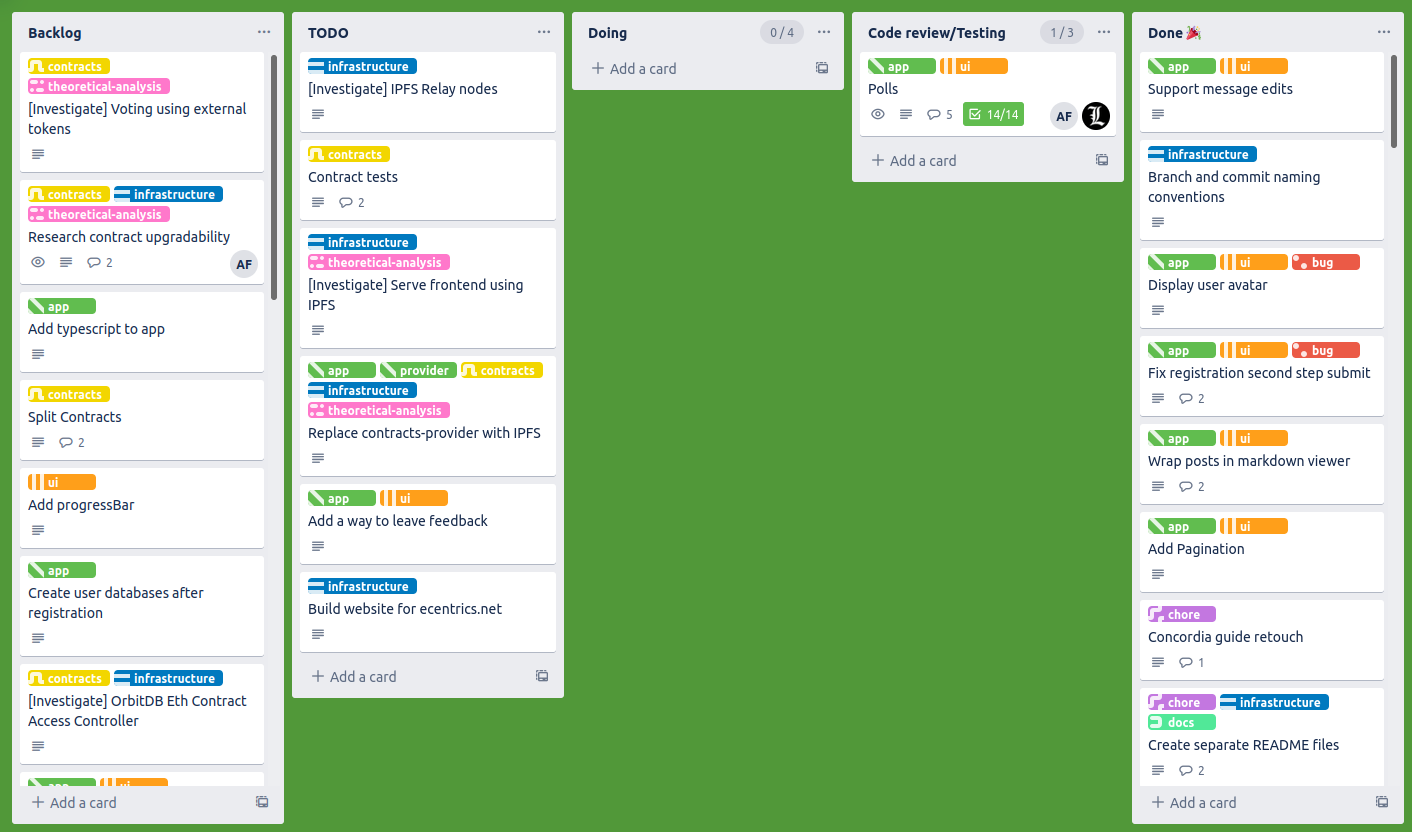
\includegraphics[width=.8\textwidth]{assets/figures/chapter-4/4.1.implementation-methodology-kanban.png}
    \caption{Στιγμιότυπο οθόνης της διαδικτυακής υπηρεσίας Trello που χρησιμοποιήθηκε για την υλοποίηση του Scrum}
    \label{figure:4.1.implementation-methodology-kanban}
\end{figure}

Κατά την διαδικασία της ανάπτυξης του κώδικα, εφαρμόστηκαν επίσης οι τακτικές που ορίζονται από το DevOps σε ό,τι αφορά το deployment των υπηρεσιών. Το DevOps ορίζει διάφορα εργαλεία που αποσκοπούν στην απρόσκοπτη, αυτοματοποιημένη και γρήγορα ενσωμάτωση του κώδικα από το στάδιο της συγγραφής μέχρι την ολοκλήρωση και εγκατάσταση. Τα εργαλεία που χρησιμοποιήθηκαν εδώ είναι:

\begin{itemize}
    \item συνεχής έλεγχος (continuous testing)
    \item συνεχής ολοκλήρωση (continuous integration)
    \item συνεχής παράδοση (continuous delivery)
    \item συνεχής εγκατάσταση (continuous deployment)
\end{itemize}

Για την υλοποίηση των τακτικών αυτών επιλέχθηκε μετά από εκτενή έρευνα η πλατφόρμα Jenkins. Το Jenkins συνδυάστηκε με την πλατφόρμα εικονοποίησης Docker ώστε να ακολουθηθούν οι τελευταίες ενδεδειγμένες πρακτικές της βιομηχανίας. Έγινε συγγραφή του αρχείου Jenkinsfile το οποίο περιγράφει με κώδικα την ροή εργασιών (pipeline) που πρέπει να ακολουθηθεί μετά από κάθε αλλαγή στον κώδικα. Η εκτέλεση του pipeline πραγματοποιείται αυτόματα από το Jenkins.

Το pipeline αποτελείται από στάδια και βήματα τα οποία φαίνονται στο σχήμα \ref{figure:4.1.implementation-methodology-jenkins-pipeline}:

\begin{enumerate}
    \item Αρχικά εκτελείται το βήμα "Version", το οποίο συλλέγει στοιχεία σχετικά με την εκτέλεση του pipeline όπως το κλαδί του κώδικα που πυροδότησε τη ροή και ποια από τα πακέτα λογισμικού που περιλαμβάνονται στο git repository περιέχουν αλλαγές.
    \item Έπειτα εκτελείται το στάδιο "TEST" το οποίο περιέχει δύο βήματα που εκτελούνται παράλληλα και πραγματοποιούν έλεγχο του κώδικα των πακέτων.
    \item Αν το κλαδί πυροδότησης είναι ένα feature branch η ροή σταματά εδώ, ενώ αν πρόκειται για ένα από τα βασικά κλαδιά (master ή develop) τότε η ροή συνεχίζει με το στάδιο "BUILD" στο οποίο εκτελούνται παράλληλα τα βήματα που χτίζουν τα docker images των πακέτων εκείνων τα οποία περιέχουν αλλαγές.
    \item Στο στάδιο "PUBLISH", αν το κλαδί πυροδότησης είναι το κύριο κλαδί παραγωγής (master), τότε εκτελούνται παράλληλα βήματα τα οποία δημοσιεύουν τα docker images που δημιουργήθηκαν στο αποθετήριο Dockerhub.
    \item Τέλος, εκτελείται το στάδιο "DEPLOY", κατά το οποίο πραγματοποιείται η εγκατάσταση των υπηρεσιών στο ανάλογο περιβάλλον, staging για το κλαδί develop και production για το κλαδί master.
\end{enumerate}

\begin{figure}[H]
    \centering
    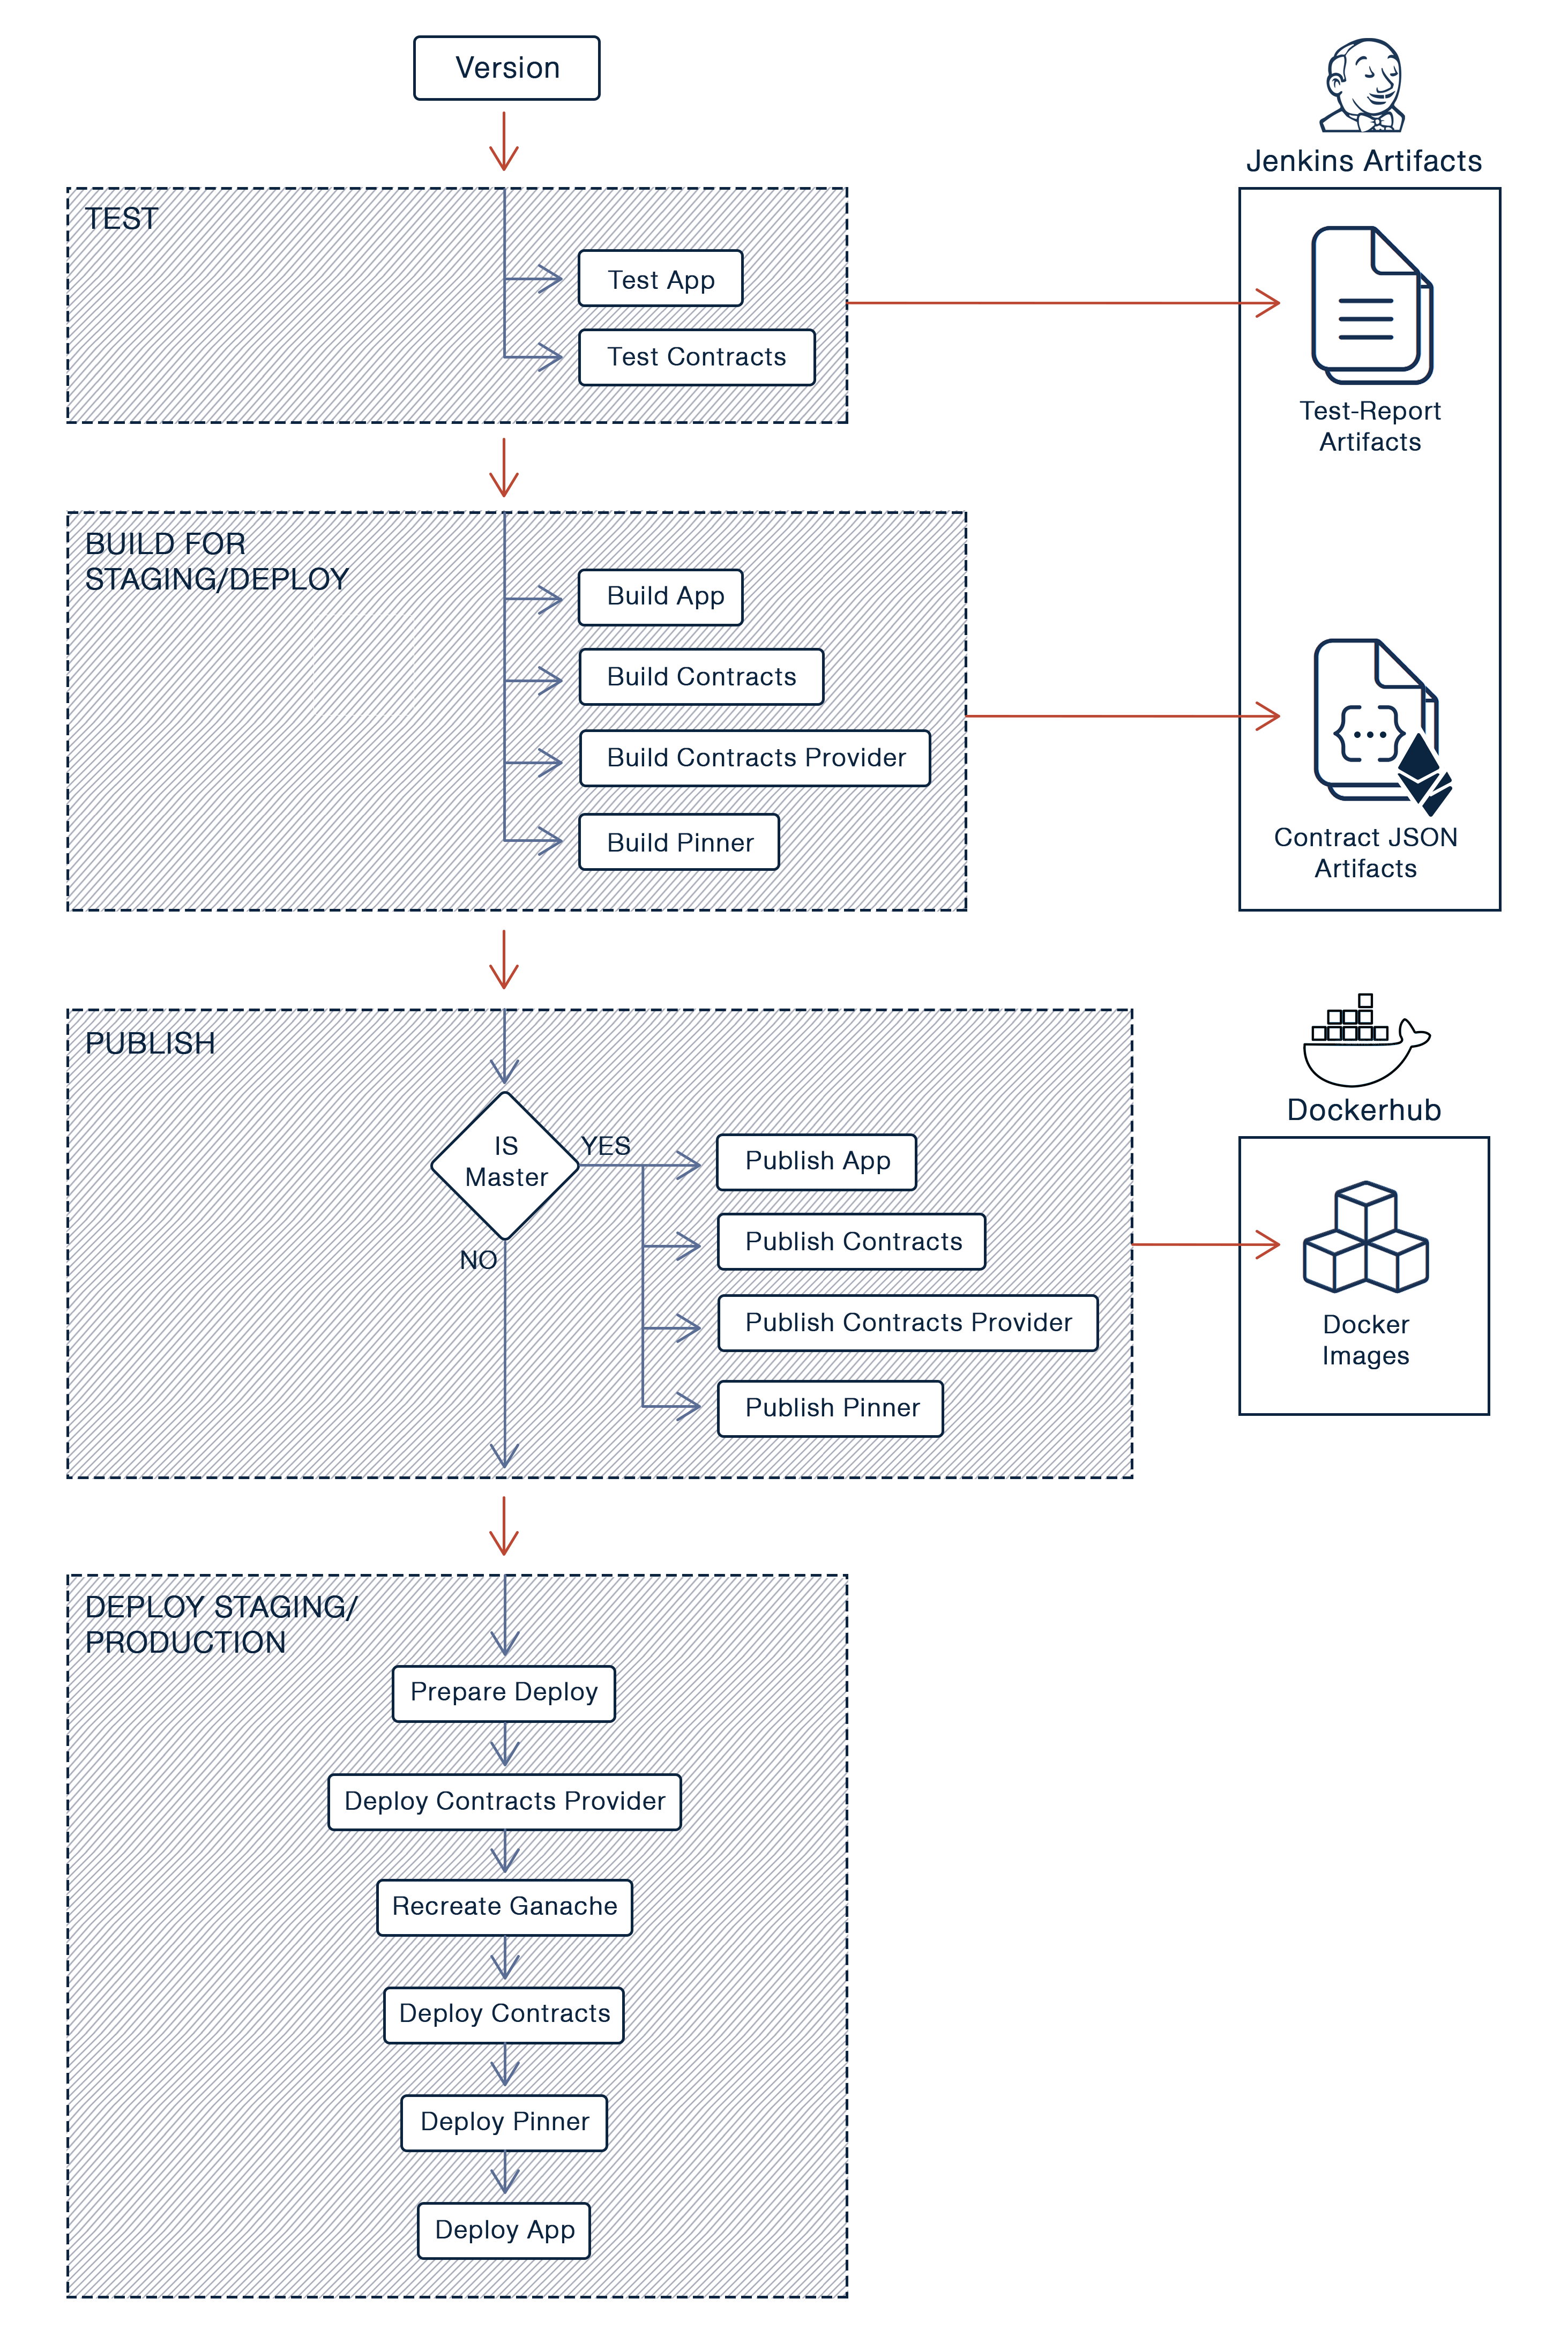
\includegraphics[width=.8\textwidth]{assets/figures/chapter-4/4.1.implementation-methodology-jenkins-pipeline.png}
    \caption{Διάγραμμα ροής εργασιών Jenkins}
    \label{figure:4.1.implementation-methodology-jenkins-pipeline}
\end{figure}

Με την χρήση του Jenkins αυτοματοποιείται με μεγάλη ευκολία ένα σημαντικό μέρος των διαδικασιών ανάπτυξης και δημοσίευσης του κώδικα. Με την χρήση του συγκεκριμένου pipeline γίνεται σίγουρο ό,τι σε κάθε αλλαγή, ασχέτως του κλαδιού ανάπτυξης ο κώδικας ελέγχεται και τα αποτελέσματα των tests είναι αποθηκευμένα και διαθέσιμα για ανάλυση. Ακόμα, για το κλαδί develop, αυτοματοποιείται η ολοκλήρωση των πακέτων και η εγκατάστασή τους σε περιβάλλον δοκιμής (staging), γεγονός που διευκολύνει σημαντικά τις συλλογικές δοκιμές από την ομάδα σε διαφορετικά περιβάλλοντα χρήσης (browsers). Τέλος, για το κλαδί master, αυτοματοποιείται η διαδικασία δημοσίευσης των docker images, μηδενίζοντας έτσι τον χρόνο που πρέπει να καταβάλουν τα μέλη της ομάδας σε αυτό.
